
\begin{aufgabe}
	
Während des Unterrichts wurde das folgende Arbeitsdiagramm für das Spannen eines Luftballons aufgenommen.

\begin{center}
	\begin{tikzpicture}[xscale=1,yscale=0.5]
		\Xachse{0}{12}{2}{Auslenkung $l$ (cm)}
		\Yachse{0}{10}{2}{Kraft $F$ (N)}
		\SPoint{2,1.7}
		\SPoint{4,3.5}
		\SPoint{6,5.0}
		\SPoint{8,7.2}
		\SPoint{10,9.0}
	\end{tikzpicture}
\end{center}

\begin{enumerate} [a)]
	\item Wie viel Verformungsenergie ist im Luftballon gespeichert?
	\item Wie hoch würde der Luftballon mit dieser Energie kommen, wenn die gesamte Verformungsenergie in potentielle Energie
		umgewandelt werden würde? (Die Masse des Luftballons ist \SI{3.2}{g})
	\item Bei einem Test haben Sie festgestellt, dass der Luftballon nur etwa zwei Meter aufsteigt. Was ist mit der restlichen Energie passiert?
		Und wie viel restliche Energie ist es?
\end{enumerate}

\end{aufgabe}

